\chapter{Requirements}\label{ch:Req}
The requirements that have been chosen for this project is listed in the following tabular \ref{tab:req}.  

\begin{table}[H]
\caption{Table of requirements.}\label{tab:req}
\begin{tabular}{|c|l|c|c|}
\hline
\textbf{Number} & \textbf{Performance requirements}  & \textbf{Desired value}& \textbf{Accuracy} \\ \hline
1 & Desired distance to a surface             & 400 mm       & $\pm$5 \% \\ \hline
2 & Detection of an object                    & $\geq$1000 mm      & -  \\ \hline
3 & Activation of the sensor at desired angle & $0\degree$          & $\pm10 \degree$  \\ \hline
4 & Drone speed                               & $\leq$ 1 m/s &   \\ \hline
 & \textbf{Functional requirements}  & \textbf{Desired value} & \\ \hline
5 & Overshoot              & $\leq$30 \% & \\ \hline
6 & Settling time           & $\leq$10 s & \\ \hline
7 & Steady state            & $\pm$5 \% & \\ \hline
8 & Sampling time          & $\geq$40 Hz   & \\ \hline
\end{tabular}
\end{table}

\section{Performance requirements} \label{sec:req}
In this section the requirements for performance that have been chosen, can be seen in table \ref{tab:req}, will be explained. %First the performance requirements and then the functional requirements. 

\begin{figure}[h]
    \centering
    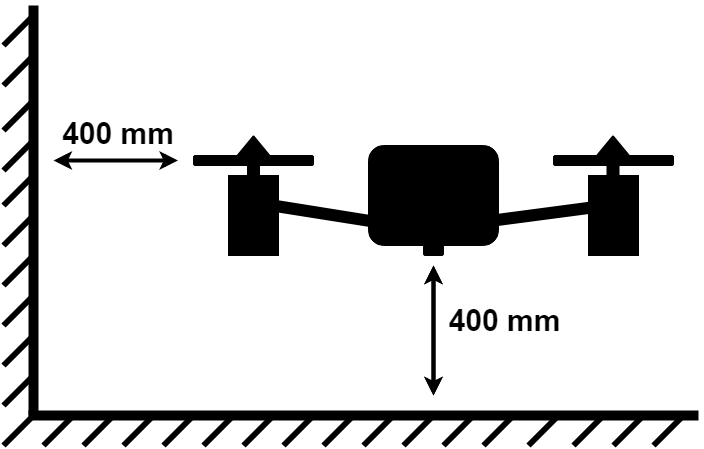
\includegraphics[width=0.70\textwidth]{figures/ch_req/figure_requirements.png}
    \caption{Figure of the requirements for the distance from the drone.}
    \label{fig:req_fig}
\end{figure}

%\subsection*{Desired distance to the floor}
%The distance to floor as seen in the table \ref{tab:req} is a fixed distance, as it is within the stable range of our sensors.


%The desired distance as seen in the table \ref{tab:req} is set,because it is necessary to avoid collision with any obstacles the drone meets on its route. These obstacles could be anything that are placed on the floor, an example of objects could be bags, chairs etc. But there are probably still some obstacles that the 400 mm might not be enough to avoid collision. However, this is just a proof of a concept, such that it would be possible to fly along side a even surface. 

%As shown in table \ref{tab:req} number 1, the desired fixed distance to the floor is 400 mm. The reason for a fixed distance is to avoid any collision with obstacles like lamps that are mounted in the celling.%The drone will avoid collision with objects like lamps in the ceiling by flying at a height at 400 mm.
%However, this is made as a proof of a concept, to make the drone fly along side a even surface. 
\subsection*{Desired distance to a surface}
The distance to a surface is set to 400 mm as a fixed distance. The distance is from the tip of the propellers to surfaces beside the drone, as shown on figure \ref{fig:req_fig}, and from the tip of the legs to the surface below, also shown on the figure \ref{fig:req_fig}. This is chosen such that the distance to the surfaces are far enough to avoid collision with either of the surfaces, and if the overshoot get to the maximum and even goes beyond that. 

\subsection*{Detection of an object}
The desired distance for detection an object is set to 1000 mm. Since the drone must be able to detect an object before the distance to the object reach the 400 mm, which is the desired distance to an object or surface. The detection of an object has been chosen to be at 1000 mm, to make it possible for the drone to stop before collision, at a reasonable speed.% From the datasheet it can be seen that the maximum distance for the chosen sensor to detect an object is 2000 mm, this mean by choosing 1000 mm it will be within the sensors range.

\subsection*{Activation of the sensor at desired angle}
The measuring angle from the sensor to the wall is chosen to be $0\degree$ with $\pm 10 \degree$. It is needed to make some variation from the $0\degree$ to make the sensor detect an object even when it is not perpendicular to the object. Therefor it is chosen to be at $\pm 10 \degree$ accuracy.

\subsection*{Drone speed}
The speed for the drone is limited to 1 m/s, this is chosen, because this will make the drone fly slowly enough to make a proof of concept for this project. This will also make it possible to follow the drones movement, and to stop within one meter. This means the drone should be able to decelerate at a rate of 1 m/s$^2$.

%The speed of the drone is limited to 1 m/s, so the drone flies slowly enough to make a proof of concept for the project. And it is still possible to follow the drones movements.

\section{Functional requirements}
Like the performance requirements were explained in \ref{sec:req}, will the focus in this section be on explaining the functional requirements.

\subsection*{Overshoot}
The overshoot of $\leq$ 30 \% is chosen to make sure the drone does not collide with an object, even if the desired distance to the wall fails. By using the 30 \% means that the distance accepted for the drone to move inside the desired distance will be at 120 mm. 
Since the overshoot and dampings ratio are dependent on each other, the overshoot can be used to find the damping ratio seen in equation \ref{eq:damping}. Where PO is the Percent Overshoot, these means the damping ratio will be 0.374 as shown in equation \ref{eq:damping}.
\begin{equation}\label{eq:damping}
   \zeta = \sqrt{\frac{(ln(\frac{\text{PO}}{100}))^{2}}{\pi^{2}+(ln(\frac{\text{PO}}{100}))^{2}}} \to \sqrt{\frac{(ln(\frac{\text{30}}{100}))^{2}}{\pi^{2}+(ln(\frac{\text{30}}{100}))^{2}}}=0.374
\end{equation}
\subsection*{Settling time}
The settling time is set to $\leq$10s, this time has been chosen to make sure the drone has time to settle in to its desired distance to a surface. It makes it possible to adjust the drones position. 
\subsection*{Steady state}
The steady state is set to  $\pm$5 \%, as it also is the accuracy to the desired distance to the wall. This also means that the steady state also need to be at this value. 

\subsection*{Sampling time}
The sampling time is set to 40 Hz, to make sure that there are enough sampling to ensure the phase offset caused by the sampling time, is not too big.

\section{Testing of the requirements}\label{s:test_requirements}
To make sure the drone lives up to all the requirements, some test specification is needed for each of the requirements.


For requirement number one and two, as it can be seen in table \ref{tab:req}. They are each tested at the maximum distance, specified by the requirements. Additionally they are also tested at 400 mm, to make sure they hold the $\pm5 \%$ to the specific distance. 


To make sure the sensors fulfill the third requirement, is to test if the sensor still can detect an object even if the sensor is not facing the wall directly, so to test this the sensors are each turn $\pm10\degree$ from the test object.


To test the fourth requirement, the drone's speed the drone's position over time needs to be tracked.


To make sure that requirement five, six and seven are fulfilled, each of these are first simulated and then tested. To test these requirements the drones position over time will again need to be tracked, and then processed to make sure the requirements are met. 


To make sure the sampling time meets requirement number eight, a number of samples is counted and the time used is noted. By using 
these two numbers the sampling time can be calculated. 
% overshoot(%) < (distance to ground(%)) from ((max measure distance) - (distance to ground))

% Settling time: vi skal vælge en tid (for stor stettling time kan få systemet til at virke langsomt.

% Steady state error: vælges ud fra afstandes sikkerhed

% krav til hvor meget fejl som vinkel for dronen må have

% SAMME KRAV TIL VÆG
%%%%%%%%%%%%%%%%%%%%%%%%%%%%%%%%%%%%%%%%%%%%%%%%%%%%%%%%%%%%%%%%%%%%%%%%%%

%%%%%% Krav til sensor %%%%%%%%%%%%%%

% krav til hvor præcis den er.

% krav til hvor hurtige den er til læse målte værdier.

% Krav til min afstand og max afstand.


%%%%%%%%%%%%%%%%%%%%%%%%%%%%%%%%%%%%%%%%%%%%%%%%%%%%%%%%%%%%%%%%%%%%%%%%
%%%%%%%%%%% Funktional krav %%%%%%%%%%%%%%%%%%%%%%%%%%

% Krav hvornår sensoren skal aktiveres

% Krav Krav til hvilke vinkel den må aflæse værdi fra væg og gulv.

% 

%%%%%%%%%%%%%%%%%%%%%%%%%%%%%%%%%%%%%%%%%%%%%%%%%%%%%%%
% det er ikke et krav hvis dataene er taget fra et datasheet. (det er limitations)

% hvordan skal kravene tests (accepttest)

% Krav til sampling tid for sensor

% krav til sensors nøjaktrighed.
